\setmainfont{Noto Serif}
\setsansfont{Noto Sans}
\setmonofont{Noto Sans Mono}
\setstretch{1.35}

\section{ЯМР спектроскопия}
1С. Нарисуйте спектры $^1\text{H}$, $^{13}\text{C}$ и $^{19}\text{F}$ ЯМР следующих соединений: (1) $\text{CH}_3\text{CH}_2\text{OH}$, (2) $\text{CH}_3\text{CH}\text{O}$, (3) $\text{CH}_3\text{CH}_2\text{O}\text{CH}_3$, (4) $\text{CF}_3\text{H}$.
\par
2С. В спектре $^1\text{H}$ ЯМР соединения $\text{C}_{6}\text{H}_{6}\text{N}_{6}\text{O}_{6}$ присутствует одна линия с химическим сдвигом 10,2 м. д. В спектре $^{13}\text{C}$ ЯМР присутствует две линии. Определите структуру молекулы.
\par
3С. Определите структуры соединений по приведенным ниже $^1\text{H}$ ЯМР спектрам и брутто-формулам: (1) $\text{C}_{9}\text{H}_{13}\text{N}$, (2) $\text{C}_{3}\text{H}_{4}\text{F}_4\text{O}$.
\begin{figure}[h]
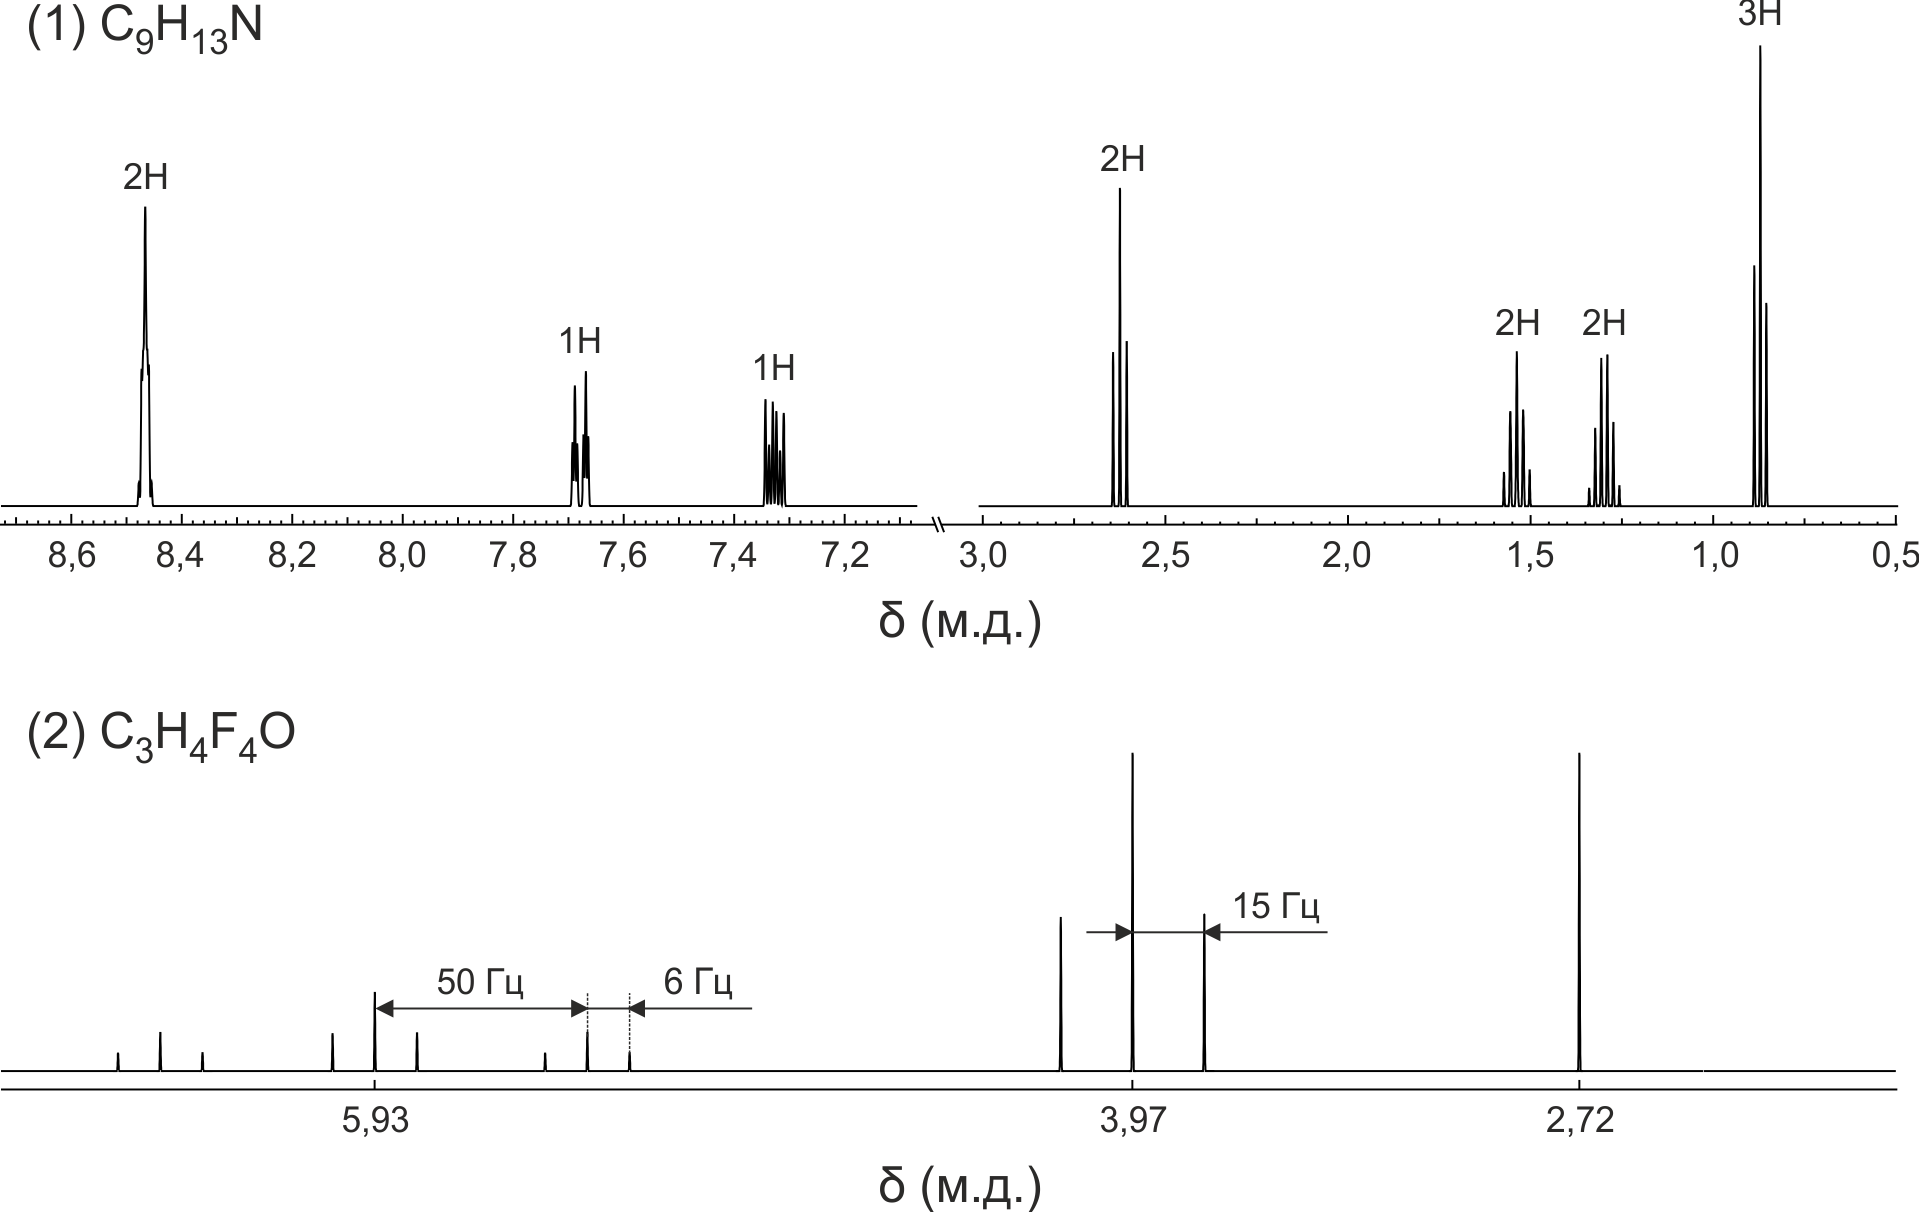
\includegraphics[width=10cm]{images/Fig_2_9_3.png}
\centering
\end{figure}
\par
\vspace{-\parskip}
4С. Определите структуры соединений по приведенным описаниям $^1\text{H}$ ЯМР спектров и брутто-формулам:\\ 
(1) $\text{C}_{3}\text{H}_{6}\text{O}$: $^1$H ЯМР (400 МГц) $\delta$ (м. д.): 5,0 (т, 4H); 2,0~(квинт, 2H);\\
(2) $\text{C}_{5}\text{H}_{11}\text{Cl}$: $^1$H ЯМР (400 МГц) $\delta$ (м. д.): 3,57 (т, 2H, $J$ = 6,8 Гц); 1,72 (дт, 2H, $J$ = 7,2; 6,8~Гц); 1,46 (м, 1H, $J$ = 6,6; 7,2 Гц); 0,88 (д, 6H, $J$ = 6,6 Гц);\\
(3) $\text{C}_{6}\text{H}_{9}\text{Br}\text{O}_{3}$: $^1$H ЯМР (400 МГц) $\delta$ (м. д.): 3,66 (c, 3H); 2,53 (c, 3H); 1,86 (c, 3H).
\par
\begin{wrapfigure}{r}{37mm} %this figure will be at the right
    \centering
    \vspace{-3.2mm}
    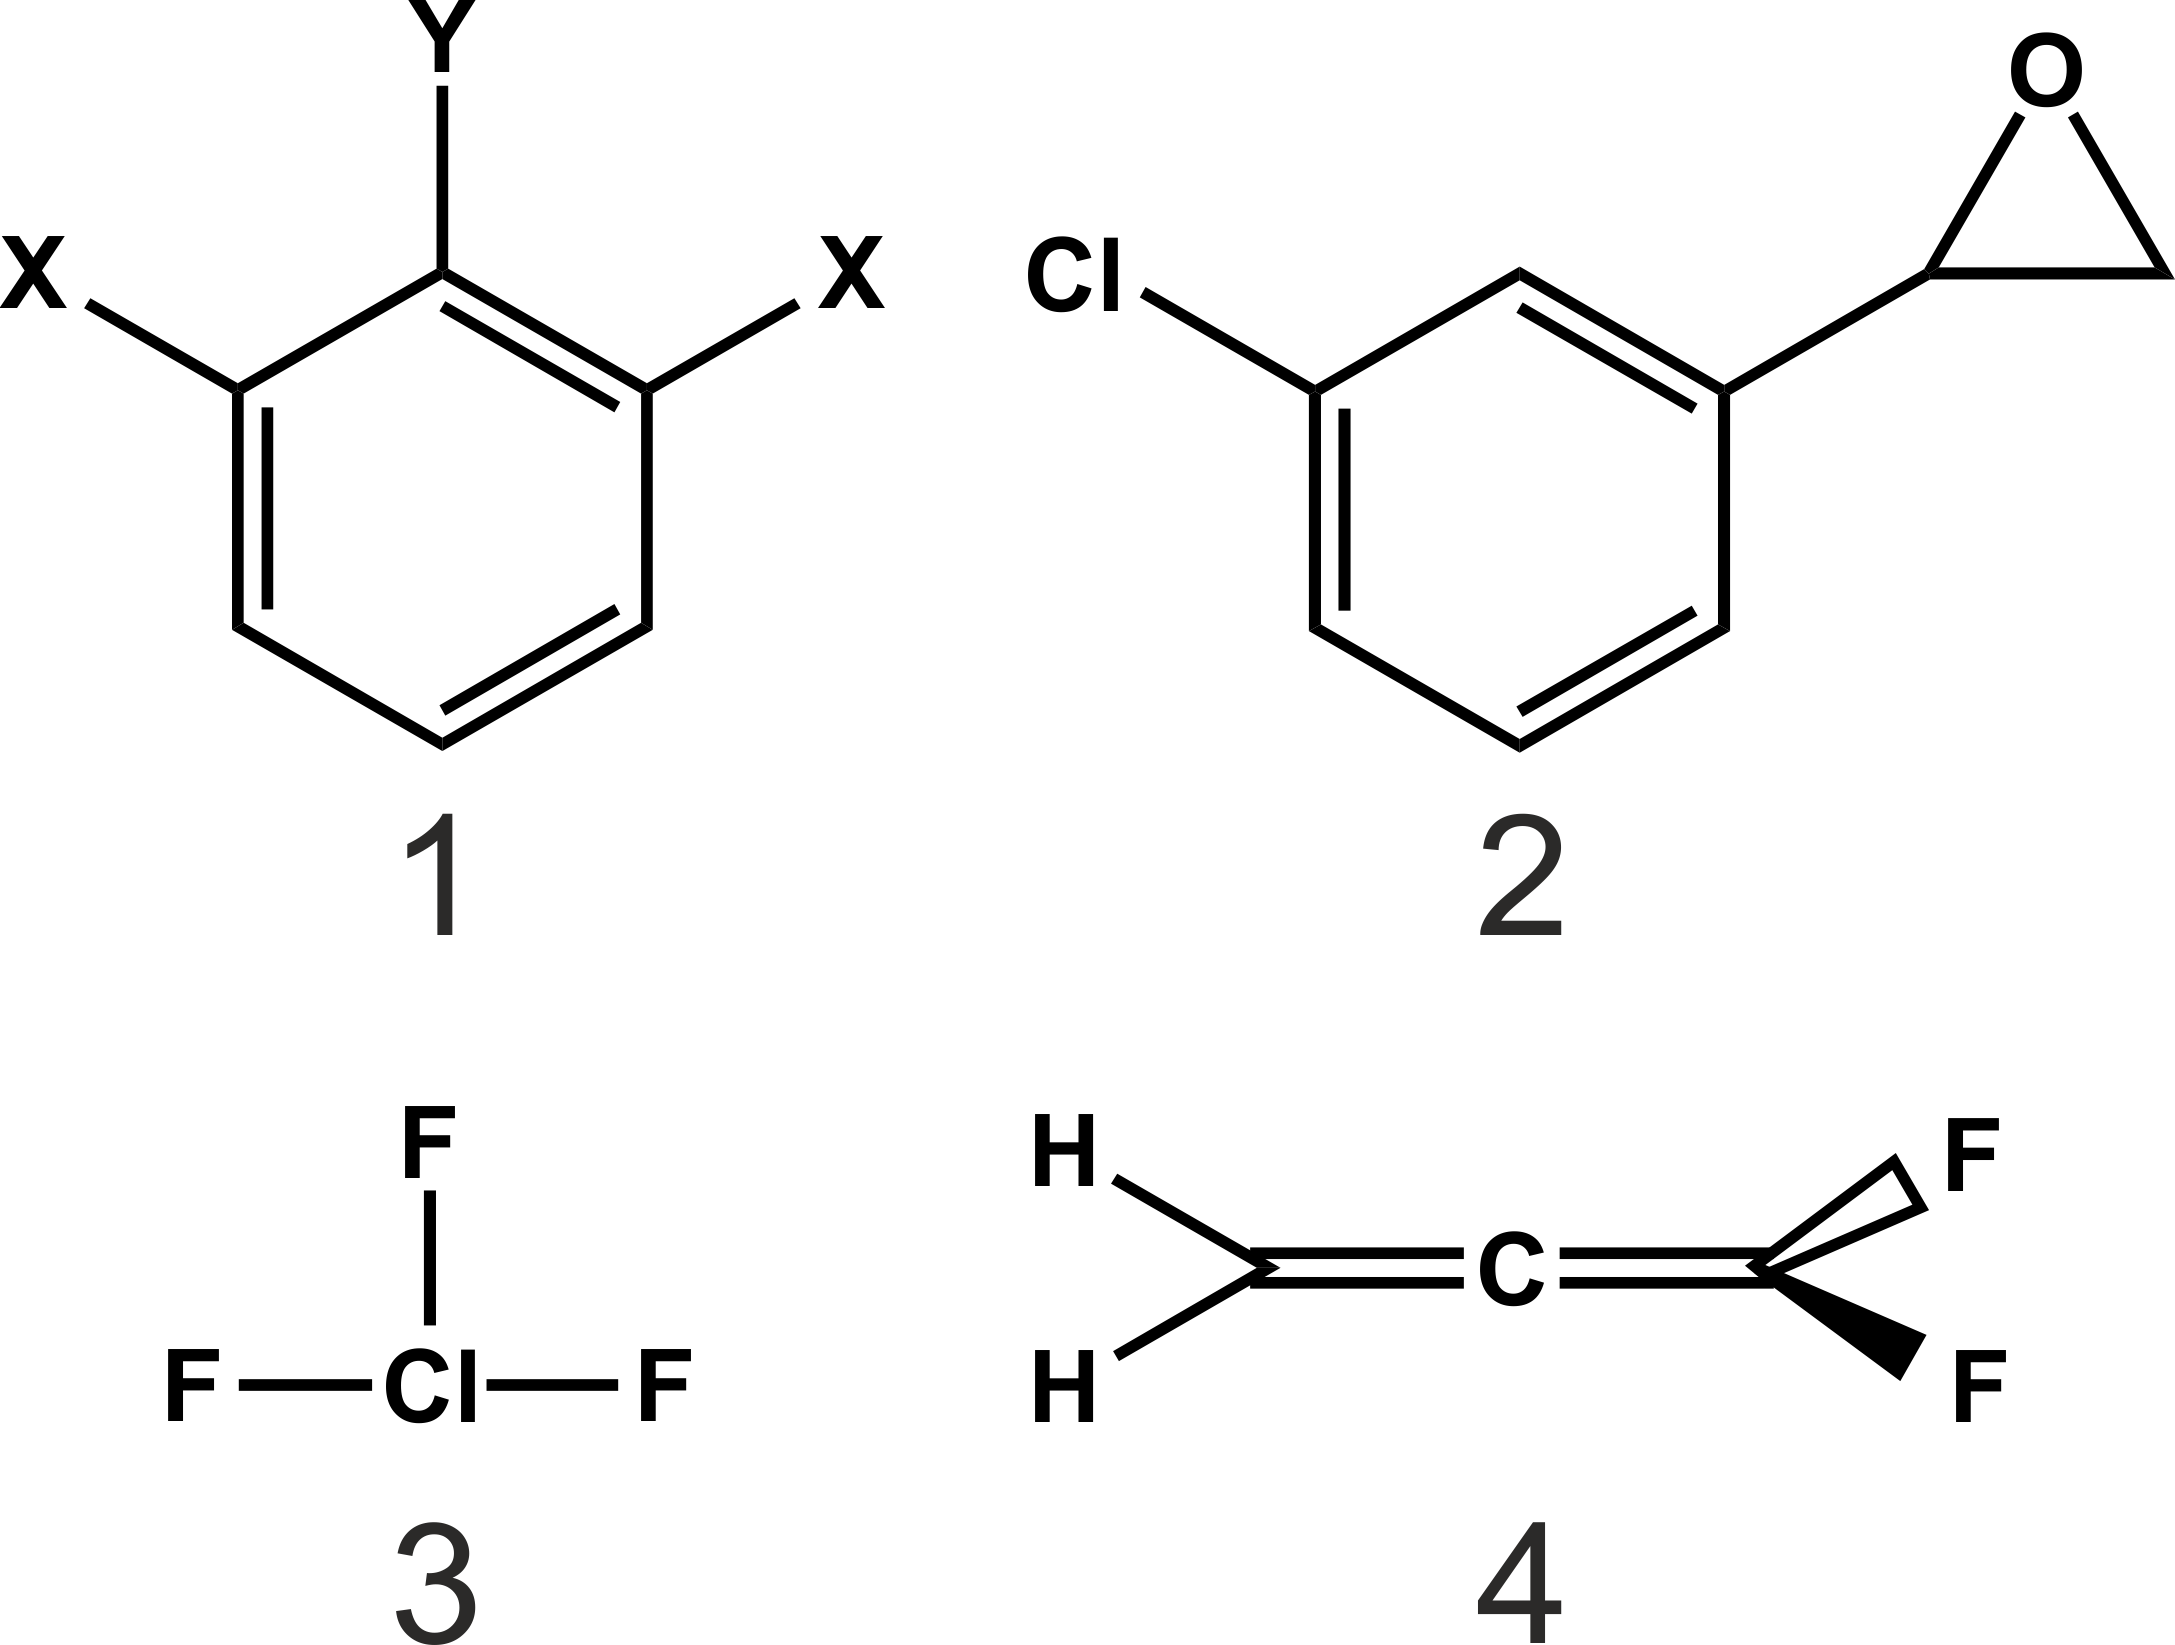
\includegraphics[width=30mm]{images/Fig_2_9_6.png}
    \vspace{-4mm}
\end{wrapfigure}
5К. Нарисуйте спектры ядерного магнитного резонанса (1) A$_2$X$_2$ системы, (2) AMX системы. Какие качественные изменения можно ожидать в спектре AMX системы при ее переходе в ABX систему? Из~приведенных на рисунке справа молекул 1–4 выберете те, которые могут соответствовать случаям (1)~и (2). Ответ аргументируйте и укажите соответствующие ядра в выбранных молекулах. Заместители X, Y не содержат магнитных ядер.
\par
6С. Для AB системы в ЯМР спектроскопии в отсутствии JJ взаимодействия расстояние между линиями равно $\delta$. При учете спин-спинового взаимодействия крайние линии стали в $n$ раз менее интенсивны центральных. Во сколько раз увеличилась протяженность спектра от крайней линии до крайней по сравнению со случаем отсутствия JJ взаимодействия.
\par
7Т. Изобразите протонный и дейтонный спектры ЯМР $\text{HD}$. Определите константу спин-спинового взаимодействия в $\text{H}_2$, считая, что она пропорциональна произведению констант СТВ рассматриваемых ядер, а линии в протонном спектре ЯМР $\text{HD}$ разнесены на 43,5 Гц.
\par
8Т. Спектр $^1\text{H}$ ЯМР некой молекулы, зарегистрированный в спектрометре с~частотой 500 МГц, состоит из двух линий с химическими сдвигами 0 и 10 м. д. Чему равна протяженность спектра $^1\text{H}$ в герцах? Для чего может быть полезным увеличить частоту ЯМР спектрометра? Чему равна протяженность спектра $^{13}\text{C}$~ЯМР в герцах, если в нем зарегистрированы линии с таким же химическим сдвигом, а ядерные $g$-факторы $^1\text{H}$ и $^{13}\text{C}$ равны 5,586 и 1,405, соответственно.
\par
9С. В спектрах $^1\text{H}$ и $^{13}\text{C}$ ЯМР молекулы с брутто-формулой $\text{C}_{4}\text{H}_{8}\text{O}_{2}$ присутствует одна линия. Определите структурную формулу данного соединения.
\par
\begin{wrapfigure}{r}{40mm} %this figure will be at the right
    \centering
    \vspace{-3mm}
    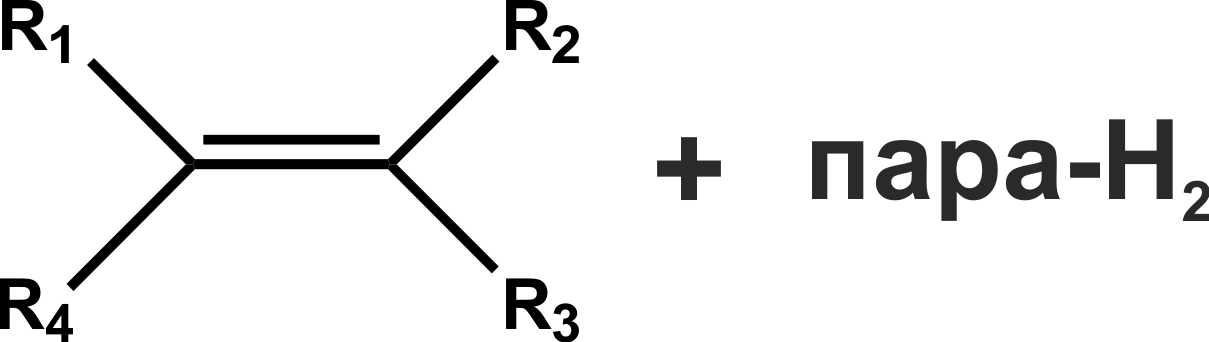
\includegraphics[width=35mm]{images/Fig_2_9_10.png}
    \vspace{-4mm}
\end{wrapfigure}
10К. Нарисуйте $^1\text{H}$ ЯМР спектр реакционной смеси непосредственно после завершения присоединения пара-водорода согласно реакции, приведенной на рисунке. Как будет выглядеть спектр, если подождать значительное время? Считайте, что заместители $\text{R}_i$, $i$ = 1–4 не содержат магнитных ядер и создают значительную разницу в химических сдвигах.
\par
11К. Определите строение соединения с брутто-формулой $\text{C}_{12}\text{H}_{18}\text{O}_{4}$, для которого были зарегистрированы следующие спектры ЯМР: $^1\text{H}$ 1,51 м. д. (с); $^{13}\text{C}$ 150,9; 85,1; 74,0; 27,9 м. д. Укажите также каким именно углеродам соответствуют приведенные значения химического сдвига. Спектр $^{13}\text{C}$ ЯМР получен в условиях подавления спин-спиновых взаимодействий с протонами.
\par
12. Спектр $^1\text{H}$ ЯМР соединения $\text{C}_{18}\text{H}_{18}$ состоит из двух синглетов с химическим сдвигом 8,9 и $-$1,9 м. д. Определите структуру данного соединения.
\par